\chapter{IRRADIANCE NETWORK FORECASTS}
\label{chap:network}

Reference other sections


Background from vincent, how it's done, limitations, possible
improvements

\section{Basic Summary}
\begin{figure}[h]
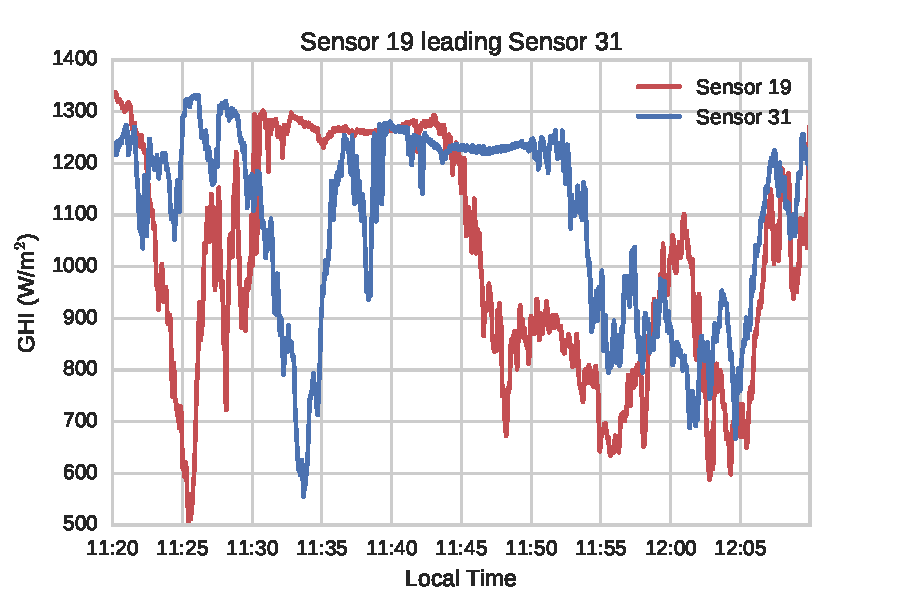
\includegraphics[width=\textwidth]{figs/leading_sens.pdf}
\caption[Example of data from one sensor predicting the output of
another]{An example of the output of sensor 19 (red) predicting what
  the output of the upstream sensor 31 (blue) in roughly 8
  minutes.}
\label{fig:leading_sens}
\end{figure}


new methods in this area

\section{Irradiance Forecast Error Metrics}
regional comparisons

time errors

standard metrics
mae vs rmse vs mbe

other metrics

make PDFs?


\subsection{Taylor Diagrams}


\section{Future Work}
velocity vectors

ensemble kalman filter

domain specific prediction

%%% Local Variables:
%%% mode: latex
%%% TeX-master: "dissertation"
%%% End:
